\documentclass[11pt]{article}
\usepackage{eacl2009}
\usepackage{times}
\usepackage{url}
\usepackage{latexsym}

\usepackage{graphics}
\usepackage[utf8x]{inputenc}
\usepackage{ucs} %sami letters\renewcommand
%\usepackage{covington} % ling examples

%\usepackage{linguex}
%{\refdash}{}
%\usepackage[T1]{fontenc}
%\usepackage{multirow}
%\usepackage{tabularx} %specified width
\begin{document}

\title{Interactive pedagogical programs based on constraint grammar}
%\author{NN}

%\author{Lene Antonsen  \and
%              Saara Huhmarniemi \and Trond Trosterud \\ University of Tromsø}

\author{Lene Antonsen\\
  University of Tromsø\\
  Norway\\
  {\tt lene.antonsen}\\{\tt @uit.no}  \And
  Saara Huhmarniemi\\
  University of Tromsø\\
  Norway\\
  {\tt saara.huhmarniemi}\\{\tt @helsinki.fi}  \And
  Trond Trosterud\\
  University of Tromsø\\
  Norway\\
  {\tt trond.trosterud}\\{\tt @uit.no}}

\pagenumbering{arabic}
 
\maketitle
%\tableofcontents

\begin{abstract}
This article presents a set of interactive pedagogical programs for North Sámi. The programs are based on a finite state morphological analyser and  a constraint grammar parser which is used for syntactic analysis and navigating in the dialogues. The analysers provide effective and reliable handling of a wide variety of user input. In addition, relaxation of the grammatical analysis of the user input enables locating grammatical errors and reacting to the errors with appropriate feedback messages. 
\end{abstract}

\section{Introduction}
This paper describes the implementation of pedagogical programs for learners of North Sámi (a Uralic language), based on a finite state transducer (fst) and constraint grammar (CG) technology. %\footnote{Thanks to the faculty of Humanities at the University of Tromsø, and the Sámi Parliament in Norway, for funding the project. The work behind the basic analysers was financed by the Research Council of Norway.}. 
The pedagogical programs are available on a web-based learning platform OAHPA!, accessible at \url{http:\\oahpa.uit.no}. There are altogether six programs: A word quiz (Leksa), a numeral quiz (Numra), basic morphological exercises (Morfa-S), morphological exercises in a sentential frame (Morfa-C), a question-answer (QA) drill (Vasta), and a dialogue program (Sahka).

The OAHPA! platform is implemented in Django, Python-based web development framework together with Mysql database.

In section 2 we describe the initial linguistic resources and the pedagogical motivation behind the programs. Section 3 presents the basic design of different parts of the programs. The fourth section shows how the CG-parser was utilised in the programs accepting free sentence input. Section 5 contains an evaluation of the programs.


\section{Background}

\subsection{Basic grammatical analysis}
The pedagogical programs in OAHPA! are based upon three pre-existing language technology resources developed at the University of Tromsø: morphological analyser/generator, a CG parser for North Sámi and a number word generator based of xfst.

Morphological analyser/generator is implemented with fst and compiled with the Xerox compilers twolc and lexc~\cite{BeesleyKarttunen:03}. Sámi languages have large morphological paradigms for each lexeme -- verbs and adjectives have more than 100 inflected forms. In addition, some of the paradigm members have a very low text frequency. Due to the limited amount of electronically available text resources, an fst analyser was used, rather than e.g. an HMM tagger \cite{Trosterud:07}. The lexicon contains 97.500 lemmas -- almost half of them proper nouns. There exist two different variants of the analyser/generator: one is tolerant, with morphological patterns based upon actual usage, and the other is normative, and adheres to the written standard.  

The morphological disambiguator is implemented in the CG-framework \cite{Karlsson:95}. The CG-framework is based upon manually written rule sets and a syntactic analyser which selects the correct analysis in case of homonymy and adds grammatical function and dependency relations to the analysis. We used vislcg3 for the compilation of CG rules. Vislcg3 is a new, improved version of the open source compiler vislcg~\cite{Visl:08}. The CG-framework is presented in section \ref{sentencefeedback}. 

\subsection{Previous accounts on parser-based pedagogical programs}

Even if many interactive parser-based programs are described in the literature, see \cite{Gamper:02,Heift:07}, very few of them are available for actual use online and most systems are in a prototype level. One of very few exception is e-tutor, a program for teaching German to foreigners \cite{Heift:01,Heift:02}, at \url{http://e-tutor.org}. E-tutor gives very good feedback to student's errors, but the student's possible input is restricted to a small, fixed vocabulary, and there is no dialogue. The grammar formalism used is Head-driven Phrase Structure Grammar (HPSG).

Vislcg3 is used in the VISL-suite of games for teaching grammatical analysis on the Internet \url{http://visl.sdu.dk}. Most of the games in VISL are based on pre-analysed sentences, but one of the programs accepts free user input in some of the 7 supported languages. The input is analysed or changed into grammar exercises~\cite{Bick:05}.

% Quoting letter from Trude Heift:
%You are right that the literature on ICALL systems is very scattered - I assume you had a look at the overview of parser-based projects described in our book (Heift & Schulze, 2007 - Routledge). There are VERY few working systems, i.e., only 3 I know of. One is a system for Japanese by Nagata (a meanwhile commercial system); a system for Portuguese - Tagarella by Meurers & Amaral which I believe covers content for an introductory course of L2 Portuguese; and the e-tutor which basically covers the entire L2 grammar of German taught in the first three university courses. I am certain that if you email the researchers, you'll get access to the systems. In addition, I know that Wolfgang Menzel at the University of Hamburg was working on a game-like system ("The Market Place") but I don't know where the project is at and whether it's in actual use by students.
%For information on the parsing aspects of the etutor, please see the following article:
%Heift, T. & Nicholson, D. (2001). Web Delivery of Adaptive and Interactive Language Tutoring. International Journal of Artificial Intelligence in Education, 12(4), 310-325.

\subsection{The pedagogical motivation} \label{pedidea}

The main goal of the development of OAHPA! was to develop a language tutoring system going beyond simple multiple-choice questions or string matching algorithms, with free-form dialogues and sophisticated error analysis. Immediate error feedback and advice about morphology and grammar 
%, as well as translations 
were seen as important requirements for the program.

In addition, the programs were designed to be flexible so that the student could choose exactly which aspect of the language and on which level of difficulty she would like to train. To better integrate the tools to the instruction, the vocabulary was designed so that it may be restricted to particular textbooks. Finally, the programs were made freely accessible via Internet.

Due to its complex morphology, Sámi languages demand a lot of practising before the student reaches 
a working level of fluency. %(tt: my suggestion)
%necessary (sh: change necessary!) skills. 
Since they are minority languages, Sámi learners often do not have enough opportunities to practise the language in a natural setting. Our freely available programs give a practical supplement to the instruction given at school or university. In addition, the dialogue program consists of everyday topics, with underlying pedagogical goals to exercise for example verb inflection, choice of correct case form or vocabulary learning. 

The student may choose between two North Sámi main dialects. Especially when training morphology, it is important that the forms that are presented for the user are the same that the ones used in the language society or taught during instruction. Still, the program accepts any correct orthographic word form provided by the student.

North Sámi is used in three countries, and therefore the programs have several metalanguages (Norwegian, Finnish, North Sámi, English). We are also considering extending the programs to other Sámi languages.

\section{Pedagogical lexicon}\label{pedlex}

\subsection{The structure of the lexicon}


All the OAHPA! -programs share a set of common resources: a pedagogical lexicon and a morphological generator that is used for generating the different word forms that appear in the programs. The dialectal variation is taken into account in lexical as well as morphological level. In addition, the morphological properties of words are used in constructing a detailed feedback on morphological errors.


%\begin{example}\label{nounsmelex}
%\begin{itemize}
%\texttt{miel0ki:miel'ki AIGI ;}
%\end{itemize}
%\end{example}

% \begin{figure}[htbp]
% \begin{center}
% \scalebox{.6}[.6]{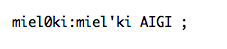
\includegraphics{presentation/img/noun-sme-lex.png}}\\
% \caption{Example of entry in the main lexicon. AIGI is the continuation class.}
% \label{nounsmelex}
% \end{center}
% \end{figure}


The pedagogical lexicon forms a collection of words that are considered relevant for the learners of North Sámi in schools and universities. The words occur in different forms in different tasks. The pedagogical lexicon contains additional information about the lemmas, such as Norwegian translation, semantic class, dialect and information about the inflection. The words in the pedagogical lexicon were collected from the key textbooks for North Sámi and the source information is included in the lexicon entry. %Cf. section \ref{set} for more information about our semantic sets. 
In addition, homonymy in both base form and inflection is dealt with using ids for lexicon entries instead of lemmas. 
The lexicon consists of 1538 nouns, 500 verbs and 194 adjectives, in addition to a small lexicon for %grammatical word classes
functional words and numbers. Figure \ref{nounlex} shows an example of an entry in the noun lexicon. \\

\begin{figure}[tbp]
\begin{center}
\scalebox{.38}[.38]{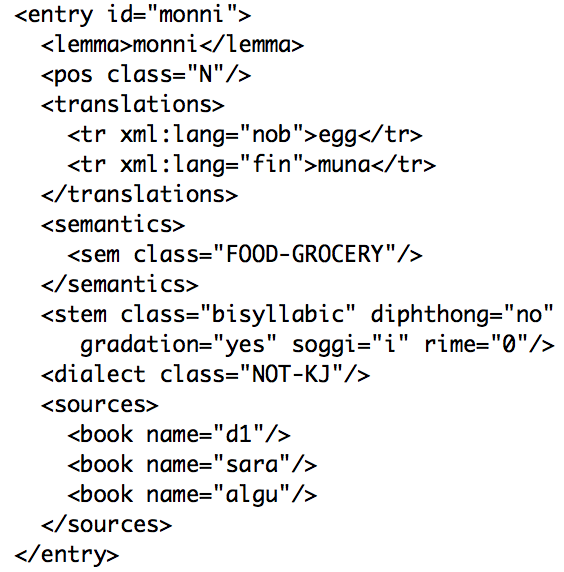
\includegraphics{presentation/img/nounlexicon4.png}}\\
\caption{An entry in the pedagogical lexicon.}
\label{nounlex}
\end{center}
\end{figure}


The word forms that are used in the program are pre-generated with a transducer that contains of the full North Sámi vocabulary, the inflectional and derivational morphology, and the non-segmental morphological processes (consonant gradation, diphthong simplification, etc.). Similar transducer is used in live analysis of user input in the programs Vasta and Sahka, which are described in section \ref{vastasahka}. Here is an example of a lexical entry (GOAHTI is the continuation class):

\begin{figure}[htbp]
\begin{center}
\begin{verbatim}
    monni GOAHTI ;
\end{verbatim}
\label{nounsmelex}
\end{center}
\end{figure}


The contents of the pedagogical lexicon as well as full paradigms for each lexicon entry are stored to the Mysql database. The database allows effective processing of queries and multiple simultaneous users. In addition, generating the word forms and storing them to the database provides better control over the inflected word forms and e.g. different dialectal forms. The handling of dialectal variation is described in the next section.


% Saara: this is all clear for anyone working in langtech.
%Some lemmas have homonymous base forms. Since they have different meanings, they belong to different semantic sets. When the student wants the translation of the lemma, it should be the translation which belongs to the particular semantic set, e.g. \textit{girdi} can be both "plane" (VEHICLE) and "pilot" (PROFESSION). Other homonymies have different inflection, and it is critical to choose the correct lemma when we are generating word forms from it, e.g. \textit{bassi} Sg Nom -- \textit{basit} Pl Nom (= holy day) and \textit{bassi} Sg Nom -- \textit{bassit} Pl Nom (= washer). We solved the problem by giving different ids to the critical entries. 

%e.g. id="girdi\_vehicle" vs. 
%id="girdi\_profession" and id="bassi\_time" vs. id="bassi\_actor".

%It works well as long as working with semantic classes, but if the user chooses "all" or a book, then he will not understand why the program doesn't accept his suggestions, e.g. "pilot" for \textit{girdi}. The solution is that the system then looks for the lemma, instead of the id.

\subsection{Handling the dialectical variation}\label{dialect}

%sh: the wordings are not very good here. what source file? how are the lines selected? Explain KJ and GG!

When generating sentences or providing the correct answers for the user, we wanted to control the selection of word forms to allow only normative forms in the correct dialect. On the other hand, the live analyser used for the analysis of the user input should be tolerant  and accept all correct variants of the same grammatical word. Therefore we compiled two different analysers/generators, one normative but variation-tolerant transducer for analysing the input, and two strict ones for different dialects for sentence generation.

The dialectal variation was in the source code (lexc) in one of the following ways:

\begin{itemize}
\item[(a)] NOT-KJ (not generate for KJ-dialect) 
\item[(b)] NOT-GG (not generate for GG-dialect)  
%\item[(c)] NG (not generate for any dialect)
\end{itemize}

Figure \ref{smelex} contains an example of how the dialectal information is handled in the lexicon file. We also marked entries in the pedagogical lexicon-files with NOT-KJ and NOT-GG, as in Figure \ref{nounlex}. This system can easily be expanded with more dialects.

\begin{figure}[htbp]
\begin{center}
\scalebox{.49}[.49]{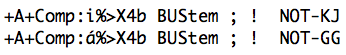
\includegraphics{presentation/img/smelex3.png}}\\
\caption{Handling of dialectal variation in the lexicon.}
\label{smelex}
\end{center}
\end{figure}

\subsection{Feedback on morphological errors}\label{mfeedback}

The inflectional information of words contained in pedagogical lexicon is used for generating feedback to the student. If the user does not inflect the lemma correctly, she can ask for hints about the inflection, and try once more, instead of getting the correct answer straight away. 

The feedback messages are determined by the combination of morphological features in the lexicon and the inflection task at hand. Consider a part of the feedback specification in the Figure \ref{feedbacknouns}. It specifies the morphological rule that there is a vowel change in illative singular for bisyllabic nouns that end with the vowel \textit{i}. The corresponding feedback message instructs the user to remember the vowel change.

\begin{figure}[htbp]
\begin{center}
\scalebox{.5}[.5]{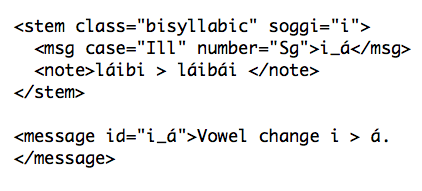
\includegraphics{presentation/img/morphfeedbackEng.png}}\\
\caption{The features in the lexicon are used to determine the correct feedback message, in this case the message is "Vowel change i $>$ á".}
\label{feedbacknouns}
\end{center}
\end{figure}

The feedback may consist several parts so that the user also receive information about e.g. stem class. All the feedback messages that match the feature definition in the given task, are collected and given to the user in a specified order. 

%\begin{figure}[htbp]
%\begin{center}
%\scalebox{.55}[.55]{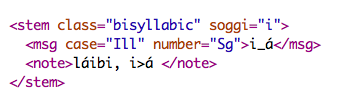
\includegraphics{presentation/img/feedback_nouns.png}}\\
%\caption{The features in the lexicon are used to give message tags. Here the message tag is "i\_á". From \texttt{feedback\_nouns.xml}.}
%\label{feedbacknouns}
%\end{center}
%\end{figure}
%
%\begin{figure}[htbp]
%\begin{center}
%\scalebox{.53}[.53]{
\includegraphics{presentation/img/messages.png}}\\
%\caption{Feedback to the user is generated from the message tags. Here for the message tag "i\_á". From \texttt{messages.xml}.}
%\label{mess}
%\end{center}
%\end{figure}
%In the example in Figures \ref{feedbacknouns}, the correct illative Sg word form of \textit{mielki} is \textit{mielkái}. %As we see in Figure \ref{nounlex}, this lemma has the feature \texttt{only-sg}, which means that we generate the lemma only in singular, even if it according to the main lexicon, also may be used in plural. This information is for pedagogical purposes; it is not that natural to use the plural form of a mass noun for a student on a lower level.



\section{CG-parser in live analysis programs Vasta and Sahka}\label{vastasahka}

%\subsection{Morfa -- word inflection}
%This is a drill made to train morphological patterns. It draws lemmas from the pedagogical lexicon at random, and the student has to answer with the word form. 

%The student can restrict the sets to certain morphosyntactic features, like Part of Speech (verbs, nouns, adjectives and numerals), and for the three first of them, it can be restricted to bisyllabic, trisyllabic and contracted stems. She can also restrict the vocabulary to certain textbooks.

%We have made two versions of the drill: Morfa-S is a bare morph-drill with singleton words. Morfa-C is a contextual morph drill, which gives matrix questions, in order to strengthen the linguistic context. After submitting the final version of the answers, the student gets a score, and a comment connected to the score.

\subsection{Overview}

In the live analysis games Vasta and Sahka, the user is allowed to formulate the full answer sentence freely. The challenge for the program is to accept different kind of correct answers and for example allow word order changes and usage different kinds of conversational particles which are typical for Sámi.

The technology used for grammatical analysis and error detection is vislcg3. The reason for choosing CG as the parser platform was that it is robust enough for handling unconstrained input, and at the same time accurate enough to identify errors. The program contains manually written, context dependent rules, mainly used for selecting the correct analysis in case of homonymy. Each rule adds, removes, selects or replaces a tag or a set of grammatical tags in a given sentential context. Context conditions may be linked to any tag or tag set of any word anywhere in the sentence, either locally (in a fixed subdomain of the context) or globally (in the whole context). Context conditions in the same rule may be linked, i.e. conditioned upon each other, negated or blocked by interfering words or tags. Vislcg3 is documented at \cite{Visl:08}. Grammars for Danish and Norwegian based on CG achieve very good F-scores \cite{Bick:03}.

The answer provided by the student is first passed to a morphological analyser (described in section \ref{pedlex}) and then analysed with vislcg3. (sh: add overall description here)

\begin{figure}[htbp]
\begin{center}
\scalebox{.48}[.43]{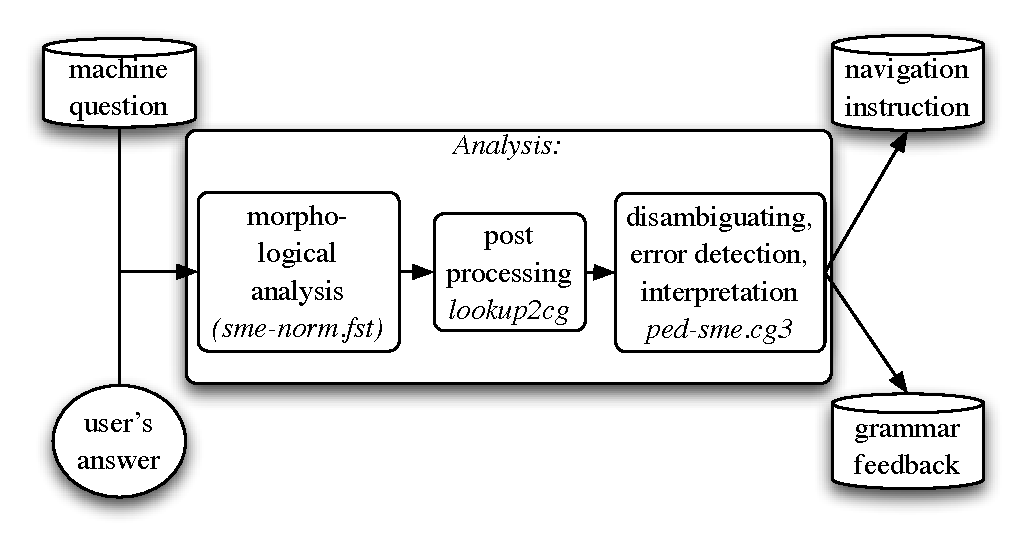
\includegraphics{presentation/img/qa2.pdf}}
\caption{An overview of the analysis process.}
\label{qasystem}
\end{center}
\end{figure}


%\begin{itemize}
%\item Level 1: verb only in present tense, logical cases
%\item  Level 2: verb in past tense, and some verbs with oblique cases, use of postpositions, questions in which the student has to answer with case in plural,  numerals and collective numerals in nominative
%\item  Level 3: grade: numerals inflected in cases, conditional, time expressions, collective numerals
%\end{itemize}
%\vspace{0.5cm}


%\begin{figure}[htbp]
%\begin{center}
%\scalebox{.4}[.4]{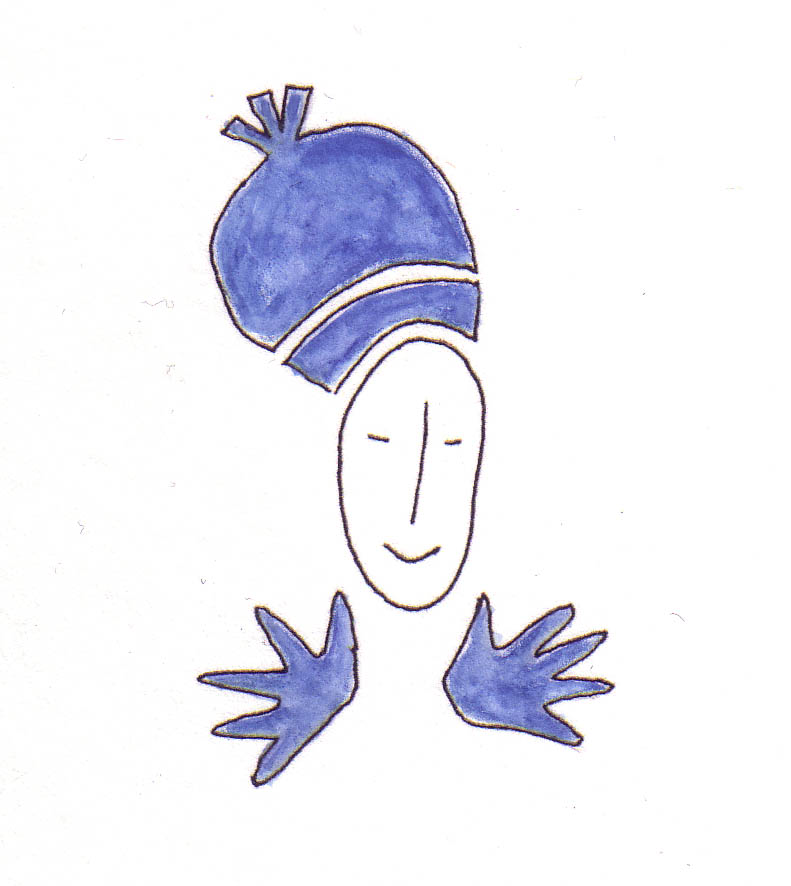
\includegraphics{presentation/img/vasta.png}}\\
%\caption{Vasta, at \textit{http://victorio.uit.no/oahpa/vasta/}}
%\label{vasta}
%\end{center}
%\end{figure}	

\subsection{The open QA drill -- Vasta}
In between the "natural" dialogues, mimicking real life dialogues, and the pure grammar training session, inquiring paradigm forms, we have made  a question-answer drill. The drill has two question types: Yes/no questions and wh-questions. 

There are two motives for making this program type. First, our tailored dialogues run the risk of getting quickly consumed. With a QA drill we may generate an indefinite number of questions. Second, the students need to automate the question-answer routine -- answer with the correct verb, inflect the finite verb correctly and choose the correct case form.

The questions are generated and presented for the user one at the time. The question and answer are analysed together, and the student gets feedback, as described in \ref{sentencefeedback}. The question matrices are marked with a difficulty level.  The student may formulate the answer freely, but she has to use a full sentence (containing a finite verb), and use the same verb as in the question. There are 111 matrix questions.

Figure \ref{questionv} contains an example of sentence matrix that is used in the sentence generator.

\begin{figure}[htbp]
\begin{center}
\scalebox{.5}[.5]{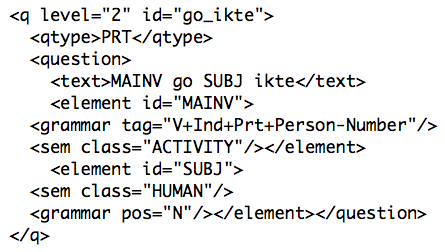
\includegraphics{presentation/img/question_vasta2.png}}\\
\caption{Example of generating if questions (MAINV question-particle SUBJ yesterday).}
\label{questionv}
\end{center}
\end{figure}

%\begin{figure}[htbp]
%\begin{center}
%\scalebox{.5}[.5]{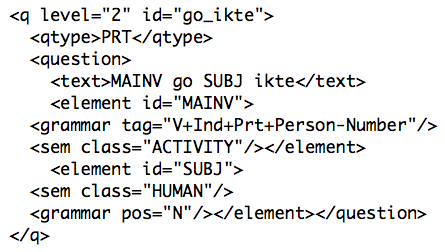
\includegraphics{presentation/img/question_vasta2.pdf}}\\
%\caption{Example of generating if questions (MAINV question-particle SUBJ yesterday).}
%\label{questionv}
%\end{center}
%\end{figure}
%
%\begin{figure}[htbp]
%\begin{center}
%\scalebox{.5}[.5]{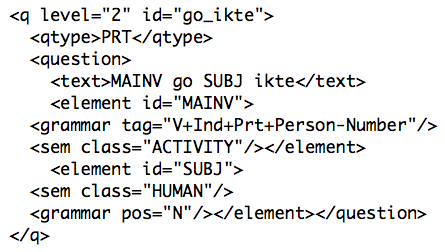
\includegraphics{presentation/img/question_vasta2.jpg}}\\
%\caption{Example of generating if questions (MAINV question-particle SUBJ yesterday).}
%\label{questionv}
%\end{center}
%\end{figure}

The question matrix contains two types of elements: constants and grammatical units. The constants such as \textit{go} and \textit{ikte} in the Figure \ref{questionv} are present in each generated sentence as such, whereas grammatical units allow more variation. Both the inflection and the content of the grammatical units may vary from question to question, and from program to program. For example, in the question in Figure \ref{questionv} the MAINV is fixed to past tense, but the person and number inflection may vary freely. In addition, certain elements such as the sentence subject (SUBJ) have default inflection in nominative, but the default inflection may be overridden. The selection of words for the sentence is constrained by semantic sets. Semantic sets are also used as an option in the word quiz (Leksa).
%There are ordinary sets and supersets, and we choose which one suits best for the particular question/task, e.g. the big superset HUMAN with all lemmas for human beings, or a smaller subset, like PROFESSION. In Figure \ref{semset} is a definition of a superset. 
%
%%sh: this figure seems to have a lot of space on the top..
%\begin{figure}[htbp]
%\begin{center}
%\scalebox{.6}[.6]{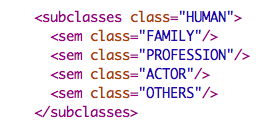
\includegraphics{presentation/img/semantic_set.png}}\\
%\caption{Some of the semantic sets are supersets, consisting of subsets. From \texttt{semantic\_sets.xml}.}
%\label{semset}
%\end{center}
%\end{figure}

The sentence generator handles agreement e.g. between subject and the main verb. The agreement may be explicitly marked between any two elements, which indicates that the two elements share the same number and person inflection.

In addition to generating questions, the sentence generator is used for generating answer templates in the contextual morphology game (Morfa-C). In this case, the sentence generator takes into account the agreement inside a sentence, but also the content and agreement between the question and the answer. For example, the person and number inflection in the answer is restricted by the question. We chose not to accept an inclusive interpretation of the pronouns in Pl1 and Du1, because we wanted the student to exercise also 2. person verb inflection. Table \ref{QA} shows how the question Person-Number (QPN) Sg1 requires answer Person-Number (APN) Sg2, and so on. Pl1 as an answer to Pl1 is thus not accepted by the system.\\


\begin{table}[htdp]
\caption{Provided question-answer agreement.}
\begin{center}
\begin{tabular}[t]{ll|ll|ll}
QPN &APN &QPN &APN &QPN &APN \\
\hline
Sg1 &Sg2 &Du1 &Du2 &Pl1 &Pl2 \\
Sg2 &Sg1 &Du2 &Du1 &Pl2 &Pl1 \\
Sg3 &Sg3 &Du3 &Du3 &Pl3 &Pl3 \\
\hline
\end{tabular}
\end{center}
\label{QA}
\end{table}

The analysis of the student's answers as well as the tutorial feedback are common to both Vasta and Sahka. They are explained in the following sections \ref{sentencefeedback} and \ref{tutorial}. 


\subsection{Syntactic analysis of the student's answer} \label{sentencefeedback}


%\textit{Maid don lohket ikte?} (What did you read yesterday?)
%\begin{itemize}
%\item \textit{Mun han lohken ollu áviissaid.} (I PART read many newspapers.)
%\item \textit{Ikte mun gal lohken buori girjji.} (Yesterday I PART read a good book.)
%\item \textit{In lohkan maidege.} (I did not read anything.)
%\item \textit{Ikte in lohkan.} (Yesterday I did not read.)
%\end{itemize}
%But the answer may contain grammar errors:
%\begin{itemize}
%\item \textit{Mun lohket ollu áviissaid.} \\ $\rightarrow$ Remember agreement between subject and verbal.  
%\item \textit{Mun lohken ollu áviissat.} \\ $\rightarrow$ There should be an accusative in your answer. 
%\item \textit{Don lohket ollu áviissaid.} \\ $\rightarrow$ Are you sure that you answer with the correct person?  
%\end{itemize}

The answer provided by the student is first passed to a morphological analyser (described in section \ref{pedlex}) and then analysed with vislcg3. The question mark is exchanged for a special symbol ("qst" QDL), cf. figure \ref{iktelohken}. Instead of a sentence delimiter, we want to be able to refer to the question and the answer separately in the rules.

\begin{figure}[htb]
\begin{center}
\scalebox{.53}[.45]{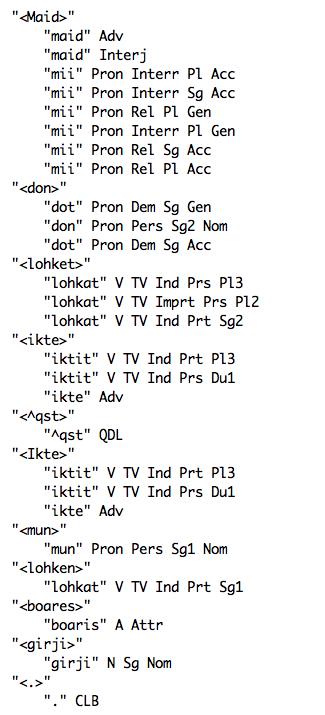
\includegraphics{presentation/img/iktelohken3.png}}
\caption{Between analysis and disambiguation.}
\label{iktelohken}
\end{center}
\end{figure}

The question and the answer are merged, and given to the analyser as one text string. We use a ruleset file which disambiguates the student's input only to a certain extent, because there will probably be grammatical and orthographic errors. The last part of the file consists of rules for giving feedback to the student's grammatical errors, and rules for reacting to the student's answer and navigating to subsequent question in the dialogue. How the feedback and navigation instructions are generated is explained in sections \ref{tutorial} and \ref{navigation}.


\subsection{Tutorial feedback} \label{tutorial}

% sh: is this correct now? I think an example sentence -answer pair would be good here.

Tutorial feedback provides the student feedback about the grammatical errors. For example, Figure \ref{cg3} presents a CG rule for assigning a grammatical error tag (CG tag \textit{\&grm-missing-Acc}) when there is no accusative found in the user input although the question requires the usage of an accusative form. In this case, requirement is based on the case of the interrogative pronoun that is used in the question. However, if the user answer is negative, the grammatical error tag is not assigned.
%, if the question is not asking for a verb, e.g. "What do you do?" (WORK-V)

\begin{figure}[htbp]
\begin{center}
\scalebox{.41}[.41]{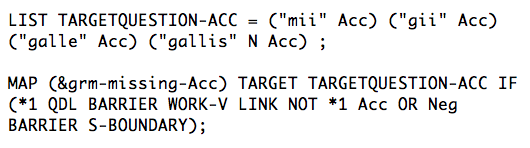
\includegraphics{presentation/img/pedcg3ny.png}}
\caption{Rule assigning missing Acc -tag.}
\label{cg3}
\end{center}
\end{figure}

Figure \ref{maidlohket} shows how the vislcg3 file has disambiguated and added the error tag about a missing accusative to the analysis from Figure \ref{iktelohken}. The error tag is used for generating feedback for the student. 

\begin{figure}[htbp]
\begin{center}
\scalebox{.47}[.47]{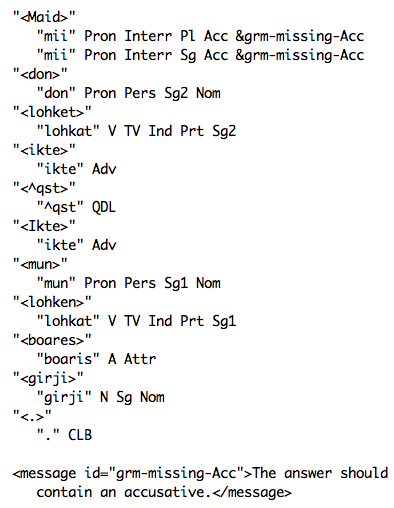
\includegraphics{presentation/img/vasta_feedback2.png}}
\caption{QA with missing Acc -tag added because the object \textit{girji} is in nominative (What did you read yesterday? Yesterday I read an old book-SgNom).}
\label{maidlohket}
\end{center}
\end{figure}

%\begin{figure}[htbp]
%\begin{center}
%\scalebox{.45}[.45]{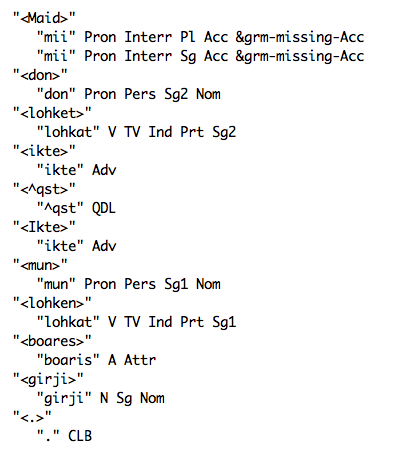
\includegraphics{presentation/img/maid_lohket_ikte3.png}}
%\caption{The grammarerrortag is added to the interrogative pronoun. (What did you read yesterday qst Yesterday I read an old book (Nom instead of Acc)). Output of vislcg3 grammar file \texttt{sme-ped.cg3}.}
%\label{maidlohket}
%\end{center}
%\end{figure}
%
%\begin{figure}[htbp]
%\begin{center}
%\scalebox{.48}[.48]{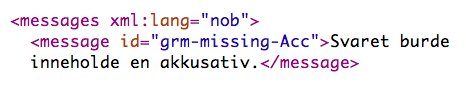
\includegraphics{presentation/img/messages_vasta2.png}}
%\caption{The grammarerrortag generates tutorial feedback. The feedback may be generated in different languages, here in Norwegian.}
%\label{messv}
%\end{center}h
%\end{figure}

The most difficult problem for the grammatical analysis are the student's misspellings. A misspelling may be left unrecognized in the analysis or it can produce another word form for the same lemma, or from some other lemma. 

When the word form is not recognized during the analysis, the feedback message to the student points to the unrecognized word form asking the student to check the spelling. To the extent that misspellings are the most common type of errors, the current feedback does not provide enough instructions for the student to improve the spelling. However, in order to give better feedback to certain misspellings, we have added e.g. place names with small initial letter to the fst, together with an error tag, so that the student gets a precise feedback. We will implement more that kind of rules and consider usage of a spell checker to help the student to find the correct word form.

%\textit{The word form is not in our lexicon, can it be a spelling error?}. 
% sh: let's give examples of something that we can do well.

For misspellings that produce another word form of the same lemma, we have written rules that are based on the grammatical context. The real problem emerges when the spelling error gives rise to an unintended lemma. Then the challenge is to give a feedback according to what the student thinks she has written. In this case, feedback has to be tailored using the knowledge about the student’s interlanguage. We have created sets for typical unintended lemmas. Combined with contextual rules we can then give the user a good feedback due to the misspelling instead of the unintended lemma.

E.g. if the student uses the Sg2 form of the main verb after the negative verb, instead of the correct ConNeg form, then the errouneous form can be a ConNeg form of a derivated verb, and the normal feedback will be: "You should answer with the same verb as in the question." The student will not understand this, because she thinks that the word form in the answer is an instance of the same verb. The solution was to generate all these forms of the verbs in the questions, make a set of them, and make a rule for in the right context, give the feedback: "The negative form is not correct." 


%\begin{itemize}
%
%\item \textbf{Locative singular without consonant gradation} \\
%The locative singular form has the suffix -s and usually consonant gradation, compared to the base form. In our pedagogical lexicon there are 1512 nouns. By adding the suffix \textit{-s} directly to the stem without consonant gradation, the result is in 57 \% of the cases a correct but unintended word form (possessive suffix in Sg3 -- e.g. \textit{viessus} instead of \textit{viesus}). Only 0,5 \% of the resulting word forms are unintended new lemmas, e.g. adverbs \textit{eanas  (eatnamis)} or verbs, e.g \textit{čogus (čohkumis)}.
%
%The possessive suffices are quite seldom used by students at lower levels, so if it does not fit to the context, one can safely assume that she has meant locative, and give feedback according to that. 
%
%\item \textbf{Illative singular without diphthong simplification and vocal change}\\
%The illative singular form has the suffix \textit{-i} or \textit{-ii} and often  diphthong simplification and vocal change. Some words have consonant gradation. By adding the suffix directly to the stem, we get 2,3 \% unintended lemmas, mostly verbs in past tense Sg3, e.g. \textit{báddii}  (pro \textit{báddái}). Generally, one man consider identifying problematic word pairs and make feedback for each of them, asking the student if she meant the other member of the pair, especially when we are not expecting one more finite verb.
%\newpage
%\item \textbf{Incorrect negative verb form}\\
%When the verb in the question is in Sg2, a common error is that the student use the Sg2 form of the verb after the negative verb, instead of the correct ConNeg form, e.g. \textit{Logat go áviissa? In logat (loga) áviissa.} The correct form is in the parentheses. The problem is that the errouneous form is a ConNeg form of another verb, \textit{logadit}, and the normal feedback will be: "You should answer with the same verb as in the question." The student will not understand this, because she thinks that the word form in the answer is an instance of the same verb. The solution was to generate all these forms of the verbs in the questions, make a set of them, and make a rule for in the right context, give the feedback: "The negative form is not correct." 
%\end{itemize}




%\subsection{Sahka -- dialogues}
\section{The dialogue program -- Sahka}
The idea behind the dialogues is that the student may exercise North Sámi in a natural setting, and at the same time receive comments about errors. Each dialogue is made to a scenario, and each scenario has a set of underlying pedagogical goals. E.g. in the Grocery-dialogue, the scenario is a shop, and the student is telling what kind of food she wants to buy. The underlying pedagogical goal is to exercise inflecting objects in accusative.

% \begin{figure}[htbp]
% \begin{center}
% \scalebox{.4}[.4]{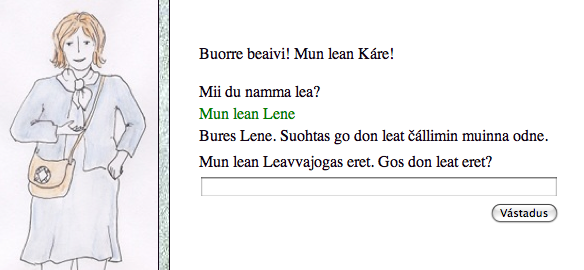
\includegraphics{presentation/img/sahka2.png}}\\
% \caption{Sahka -- the dialogue program.}
% \label{sahka}
% \end{center}
% \end{figure}

In the Get-acquainted-to-dialogues the student can choose an identity for the conversation (she chooses a picture). These identities will act as parameters for choice of comments from the computer, and for dialogue topics and dialect forms.

%\vspace{0.5cm}
%	
%Scenarios:
%\begin{itemize}
%\item Get acquainted to Hánsa -- an adult man living in Kautokeino
%\item Get acquainted to Káre -- an adult woman living in Karasjok
%\item Get acquainted to Lisa -- a girl living in Tana
%\item Get acquainted to Lemet -- a boy living in Tromsø
%\item Visit -- help to move furniture from one room to another, and have a coffee break
%\item Grocery -- buying food
%\item Comparing in the shop -- tell what is cheapest or most expensive, using adjectives in comparative or superlative
%\end{itemize}

Each dialogue consists of many branches, and different links according to the student's input. To organize them, we have made different levels (la: should be another word):

%The first utterance is a dialogue\_opening and the last utterance is a dialogue\_closing. The student can write that she wants to quit at any point during the dialogue, and by using some form of the verb \textit{heaitit} ("quit") she will navigate directly to the dialogue\_closing.

The dialogue consists of topics, and every topic starts with an opening utterance; a comment or a question. In the end of the topic, there is always a closing comment.  

Every utterance has a name, and one or more links. The choice of link is dependent upon what kind of tag the question-answer pair gets, e.g. \textit{\&dia-neg} or \textit{\&dia-pos}, or \textit{\&dia-target} to a certain word, e.g. target="hivsset", like in Figure \ref{TV}.  In Figure \ref{targetIll} we see how the \textit{\&dia-target} tag is mapped to the noun in illative. There will always be a default; in case there will not be any tag. \\

\begin{figure}[htbp]
\begin{center}
\scalebox{.40}[.42]{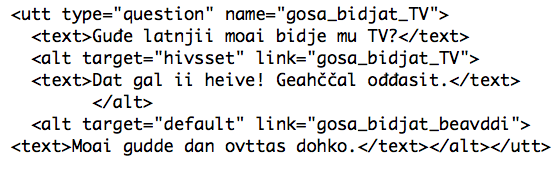
\includegraphics{presentation/img/gosabidjatTV2.png}}
\caption{The question is "In which room do we put the TV?" One of the alternatives for the navigation is due to the target tag being assigned to the lemma \textit{hivsset} (''WC``). The answer will be "That is not a good idea. Make a new try."}
\label{TV}
\end{center}
\end{figure}


\begin{figure}[htbp]
\begin{center}
\scalebox{.4}[.4]{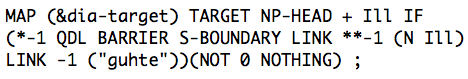
\includegraphics{presentation/img/targetIll2.png}}
\caption{A general rule, not connected to any particular question, for adding a target-tag to the NP-head in illative after a question with the interrogate \textit{guhte} + a noun in illative ( = "to which").}
%\caption{A rule for giving target-tag to an noun or pronoun in illative after a question with the interrogate \textit{guhte} + a noun in illative ( = "to which"). This a general rule, not connected to any particular question.}
\label{targetIll}
\end{center}
\end{figure}

A topic is like a module in the dialogue, and it is easy to put a new module subsequent to any topic. The linking makes it possible to make branches. Every utterance has a unique name.  

The dialogue system itself is quite simple. Only the program can make initiatives, and all the utterances from the program, are written. The program can store simple information as the student's name, place where she lives and her car type, for using in as a variable in a tailored utterance. If we were to develop the program with generating of utterances, and a more free dialogue, and also let the student take initiatives, we would have to use an analyser which maps semantic roles to the student's input, despite possible syntactic errors. In order to implement this we would need a semantically enriched lexicon.

\subsection{Navigating in the dialogue}\label{navigation}
We use the same system to navigate inside the dialogue. The input is tagged during analysis with information on whether it is interpreted as affirmative or negative, or with a target-tag, so that we can pick up e.g. a name or the essence of the answer, and use it in the next question or utterance. 

Some dialogues are branched according to how the student answers, e.g. if the question is about having a car, a positive answer will navigate to a branch with follow-up questions. In the same way an answer from the student about her age will induce a tag (Figure \ref{age}), which is used to navigate to different branches of the dialogue based on the age of the student, see Figure \ref{branch}.


\begin{figure}[htbp]
\begin{center}
\scalebox{.4}[.4]{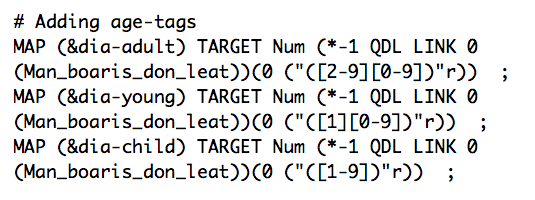
\includegraphics{presentation/img/picking_age2.png}}\\
\caption{Rules for giving age-tag to the input. Special rules for the question named Man\_boaris\_don\_leat (How\_old\_are\_you).}
\label{age}
\end{center}
\end{figure}


\begin{figure}[htbp]
\begin{center}
\scalebox{.42}[.42]{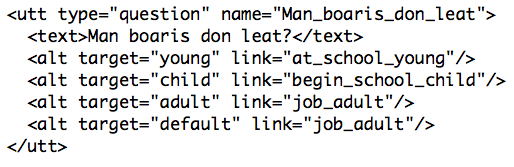
\includegraphics{presentation/img/Man_boarisEng.png}}\\
\caption{Example of how to navigate to the next question or branch, with help of the tag. The question is "How old are you?".}
% and the branches are adapted to the age of the student.}
\label{branch}
\end{center}
\end{figure}

As we see in the Figures \ref{maidlohket} and \ref{branch}, the questions in the dialogues are not generated, but written. Every question has its own unique name, so we can link to it, and it is also possible to make a rule for a special question, like in Figure \ref{age}.  



\section{Evaluation}

At the time of writing, the programs have been in public use for approximately two months. % at \textit{http://oahpa.uit.no}
All user input the word quiz Leksa, the numeral quiz Numra, the bare morphological task Morfa-S and the contextual morphology task Morfa-C has been logged from the very beginning. Unfortunately the programs Vasta and Sahka, have been logged for a couple of days only. The log contains 32475 queries (679 queries/day for the 4 programs logged the whole period), of these, approximately 600, or under 2\%, were nonsense answers. 
% (of the type \textit{asdf, aaaaa}, etc.).
% 4.2. - 1.4. = 8 x 7 = 42, 28507/42=679

\begin{table}[htdp]
\caption{Answers to the programs (Vasta and Sahka were logged at the end of the period only)}
\begin{center}
\begin{tabular}{|l|r|r|r|r|}
\hline
Program     & Correct &   Wrong &    Total &  \% \\
\hline									 
Morfa-S  &  6920   & 6323    & 13243    & 52.3 \\
Leksa    &  5659   & 4248    & 9907	    & 57.1  \\
Numra    &  3086   & 2512    & 5598	    & 55.1  \\
Morfa-C  &  1349   & 1613    & 2962	    & 45.5  \\
Sahka    &   322   &   322   &  644	    & 50.0  \\
Vasta    &   19    &   102   &  121	    & 15.7 \\
\hline
Total   & 17355  &  15120  &  32475  &  53,44\\
\hline
\end{tabular}
\end{center}
\label{log1}
\end{table}

%\vspace*{-2cm}

As can be seen from Table \ref{log1}, slightly more than half of the queries resulted in correct answers. When confronted with an error feedback, the user is offered grammatical help, and thereafter she has the possibility to give a new answer to the same query. An investigation of 1500 queries to Morfa-C showed that 444, or 30\%, were such repeated answers. Even though we have no log info of the use of the morphological feedback (section \ref{mfeedback}), our impression from classroom experience is that the users are actively using the feedback system. This indicates that what we are witnessing is a truly interactive process, where users err in half of the queries, and then follow up with a new try, possibly after having read the morphological advice from the program.

The error log for Sahka shows that one fourth of the errors are due to orthographical errors (Table \ref{log2}). Most of the "no finite verb" errors are elliptical answers, and these are not accepted, for pedagogical reasons. The remaining cases are errors where the misspelled verb is an existing word. Also for the other grammatical errors verb errors are dominating. The main goal of the program was to train verb forms in a dialogue, and the error log shows that the program is able to capture such errors.

The logs may not only be used for evaluating the programs, but also for monitoring the learning process as such. To take just one example, the Morfa logs give the error rate for each and every morphosyntactic property and stem type, thereby giving valuable information as to which parts of the verbal paradigm are the most problematic ones.

\begin{table}[htdp]
\caption{Error types for Sahka, ordered after type.}
\begin{center}
\begin{tabular}{|l|r|l|r|}
\hline
Error type & \# & Error type & \# \\
\hline												    
no finite verb    & 85 & wr. case for V-arg & 22  \\
orth. error       & 83 & wr. case after Num & 10 \\
wrong S-V agr     & 46 & wrong tense          & 9 \\
no infinite V  & 30 & no postposition      & 6 \\
wrong V choice & 24 & wrong word           & 7  \\
\hline
\end{tabular}
\end{center}
\label{log2}
\end{table}%

\section{Conclusion}

By using a sloppy version of the syntactical analyser for North Sámi, combined with a set of error-detection rules, we have been able to build a flexible CALL resource. The programs are made in a modular way, and it is easy to improve each module, and also to add more materials -- words, tasks, dialogues, levels, words from textbooks. The CG parser framework was originally chosen as parser framework for Sámi due to its extraordinary results for free-text parsing. The present project has shown that CG is well fit for making pedagogical dialogue systems as well.

The program is something quite new among pedagogical programs for Sámi, and indeed quite rare within the CALL field. %The programs are not linked to a certain chapter in a textbook, or to a certain level in the student's progression. Instead, all programs have many options, so the student can choose what to exercise, and on what level. 
The QA and the dialogue program are tolerant towards variation in student answer (not only string matching), and the random generation of tasks more or less in all of the programs, the student can use them over and over again. 

\section*{Acknowledgments}
Thanks to the faculty of Humanities at the University of Tromsø, and the Sámi Parliament in Norway, for funding the project. The work behind the basic analysers was financed by the Research Council of Norway. 



\begin{thebibliography}{}

\bibitem[\protect\citename{{Beesley and Karttunen}}2003]{BeesleyKarttunen:03}
{Kenneth R. Beesley and Lauri Karttunen}.
\newblock 2003.
\newblock {\em Finite State Morphology}.
\newblock CSLI publications in Computational Linguistics.
\newblock USA.
%Bick, Eckhard (2003-8). "A Constraint Grammar Based Question-Answering System for Portuguese". In: Fernando Moura Pires & Salvador (eds.) Progress in Artificial Intelligence (Proceedings of EPIA'2003, Beja, Dec. 2003), pp. 414-418. Springer

\bibitem[\protect\citename{Bick}2003]{Bick:03}
{Eckhard Bick}.
\newblock 2003.
\newblock {PaNoLa: Integrating Constraint Grammar and CALL applications for Nordic languages}.
\newblock Holmboe, Henrik (ed.): {\em Nordic Language Technology, Årbog for Nordisk Sprogteknologisk Forskningsprogram 2000-2004}.
\newblock {183--190},
\newblock København: Museum Tusculanums Forlag.

\bibitem[\protect\citename{Bick}2005]{Bick:05}
{Eckhard Bick}.
\newblock 2005.
\newblock {Live use of Corpus data and Corpus annotation tools in CALL: Some new developments in VISL}.
\newblock Holmboe, Henrik (ed.): {\em Nordic Language Technology, Årbog for Nordisk Sprogteknologisk Forskningsprogram 2000-2004},
\newblock {171--185}.
\newblock København: Museum Tusculanums Forlag.

%\bibitem[\protect\citename{Bick}2005b]{Bick:05b}
%{Eckhard Bick}.
%\newblock 2005b.
%\newblock {Grammar for Fun: IT-based Grammar Learning with VISL}.
%%\newblock {49--64},
%\newblock Henriksen, Peter Juel (ed.): {\em CALL for the Nordic Languages.}
%\newblock Copenhagen Studies in Language 30:49--64.

\bibitem[\protect\citename{Gamper and Knapp}2002]{Gamper:02}
{Johann Gampfer and Judith Knapp}.
\newblock 2001.
\newblock {A review of intelligent CALL systems}.
\newblock {\em Computer Assisted Language Learning} 
%\newblock {329--342},
\newblock {15(4):329--342.}
%\newblock Routledge.


\bibitem[\protect\citename{Heift}2001]{Heift:01}
{Trude Heift}.
\newblock 2001.
\newblock {Intelligent Language Tutoring Systems for Grammar Practice}.
\newblock {\em Zeitschrift fur Interkulturellen Fremdsprachenunterricht [Online] }
\newblock {6(2).}



\bibitem[\protect\citename{Heift and Nicholson}2001]{Heift:02}
{Trude Heift and Devlan Nicholson}.
\newblock 2001.
\newblock {Web Delivery of Adaptive and Interactive Language Tutoring}.
%\newblock {310--325},
\newblock {\em International Journal of Artificial Intelligence in Education}
\newblock {12(4):310--325.}

\bibitem[\protect\citename{Heift and Schulze}2007]{Heift:07}
{Trude Heift and Mathias Schulze}.
\newblock 2007.
\newblock {\em Errors and intelligence in computer-assisted language learning: parsers and pedagogues}.
\newblock Routledge studies in computer-assisted language learning 2. 
\newblock New York : Routledge.

\bibitem[\protect\citename{Karlsson et. al}1995]{Karlsson:95}
{Fred Karlsson and Atro Voutilainen and Juha Heikkilä and Arto Anttila}.
\newblock 1995.
\newblock {\em Constraint grammar: a language-independent system for parsing unrestricted text}.
\newblock Mouton de Gruyter.


%\bibitem[\protect\citename{Samuelsson and Voutilainen}1997]{SamuelssonVoutilainen:97}
%{Christer Samuelsson and Atro Voutilainen}.
%\newblock 1997.
%\newblock Comparing a Linguistic and a Stochastic Tagger
%\newblock {\em Proceedings of the 35th Annual Meeting of the Association for Computational Linguistics}.
%\newblock {Association for Computational Linguistics},
%\newblock {246--253},
%\newblock {http://www.aclweb.org/anthology/P97-1032}


\bibitem[\protect\citename{{Trosterud}}2007]{Trosterud:07}
{Trond Trosterud}.
\newblock 2007.
\newblock {\em Language technology for endangered languages: Sámi as a case study}.
\newblock http://giellatekno.uit.no/background/rvik.pdf
\newblock University of Tromsø, Norway.

\bibitem[\protect\citename{{visl}}2008]{Visl:08}
{VISL-group}.
\newblock 2008.
\newblock {\em Constraint Grammar}.
\newblock http://beta.visl.sdu.dk/constraint\_grammar.html
%\newblock Institute of Language and Communication (ISK), 
\newblock University of Southern Denmark.


\end{thebibliography}


%\begin{spacing}{1}
%\par
%\bibliographystyle{jmr} %jmr gives the second author with first name first
%\bibliographystyle{jmr}
%\thebibliography{refacl}
%\bibliographystyle{acl}


%\bibdata{refacl}
%\addcontentsline{toc}{section}{References}
%\end{spacing}

	
\end{document}

	
